\documentclass{article} % For LaTeX2e

\usepackage{nips12submit_e,times}
\usepackage{pslatex}
\usepackage{amsmath}
\usepackage{amsfonts}
\usepackage{latexsym}
\usepackage{amssymb}
\usepackage{graphicx}
\usepackage{xspace}
\usepackage{multirow}
\usepackage{array}
\usepackage{caption}
\usepackage{subcaption}
\usepackage[numbers]{natbib}

\title{Supplementary for \\ Halo, Hyperbole, and the Pragmatic \\ Interpretation of Numbers}
 
\author{
Jean Y. Wu \\
Symbolic Systems Program\\
Stanford University\\
Stanford, CA 94305 \\
\texttt{jeaneis@stanford.edu} \\
\And
Justine T. Kao \\
Department of Psychology\\
Stanford University \\
Stanford, CA 94305 \\
\texttt{justinek@stanford.edu} \\
\AND
Leon Bergen \\
Department of Brain and Cognitive Sciences\\
Massachusetts Institute of Technology \\
Cambridge, MA 02138\\
\texttt{bergen@mit.edu} \\
\And
Noah D. Goodman \\
Department of Psychology\\
Stanford University \\ 
Stanford, CA 94305\\
\texttt{ngoodman@stanford.edu} \\
}


\begin{document}

\maketitle

\section{Behavioral Experiment}

\begin{table}[h]
\begin{tabular}{| p{0.15cm}  p{8.15cm}| p{0.15cm}p{4cm} |}\hline
\multicolumn{2}{|c|}{\textbf{Scenario}} & \multicolumn{2}{|c|}{\textbf{Values for X}} \\\hline
\multicolumn{2}{|l|}{Ann and Bob are friends. They are taking the same class.} & \multicolumn{2}{|l|}{[$100$, $102$, $150$, $152$,}\\
\multicolumn{2}{|l|}{\textbf{Ann:} ``How much did the textbook cost you?"} & \multicolumn{2}{|l|}{$200$, $202$, $1000$, $1012$]}\\
\multicolumn{2}{|l|}{\textbf{Bob:} ``\{X\} dollars."} & \multicolumn{2}{|l|}{}\\\hline
\multicolumn{2}{|c|}{\textbf{Questions}} & \multicolumn{2}{|c|}{\textbf{Responses}} \\\hline
(1) & Was Bob being literal about the cost of the textbook, & (1) &[Literal / Exaggerating] \\
 & or was he exaggerating? & (2) & [Free response] \\
(2) & How much do you think the textbook actually cost? & (3) & [Likert scale] \\
(3) & How negative does Bob feel about the cost of the textbook? & (4) & [Exactly \{X\} dollars / \\
(4) & What is Bob most likely trying to communicate by saying  ``\{X\} dollars"? & & Approximately \{X\} dollars/ The textbook is expensive and Bob is not happy.]\\\hline
\end{tabular}
\caption{Textbook costs scenario}
\label{tab:myfirsttable}
\end{table}


\begin{table}[h]
\begin{tabular}{| p{0.15cm}  p{8.15cm}| p{0.15cm}p{4cm} |}\hline
\multicolumn{2}{|c|}{\textbf{Scenario}} & \multicolumn{2}{c|}{\textbf{Values for X}} \\\hline
\multicolumn{2}{|}{Ann and Bob are friends. They are walking toward Bob's car.} & \multicolumn{2}{l|}{[$100$, $102$, $150$, $152$,}\\
\multicolumn{2}{|||}{\textbf{Bob:} ``Oh no, I got a parking ticket!"} &
\multicolumn{2}{||}{$200$, $202$, $1000$, $1012$]}\\
\multicolumn{2}{|l|}{\textbf{Ann:} ``I'm sorry, how much is it?"} & \multicolumn{2}{||}{$200$, $202$, $1000$, $1012$]}\\
\multicolumn{2}{|l|}{\textbf{Bob:} ``\{X\} dollars."} & \multicolumn{2}{|l|}{}\\\hline
\multicolumn{2}{|c|}{\textbf{Questions}} & \multicolumn{2}{c|}{\textbf{Responses}} \\\hline
(1) & Was Bob being literal about the cost of the textbook, & (1) &[Literal / Exaggerating] \\
 & or was he exaggerating? & (2) & [Free response] \\
(2) & How much do you think the textbook actually cost? & (3) & [Likert scale] \\
(3) & How negative does Bob feel about the cost of the textbook? & (4) & [Exactly \{X\} dollars / \\
(4) & What is Bob most likely trying to communicate by saying  ``\{X\} dollars"? & & Approximately \{X\} dollars/ The textbook is expensive and Bob is not happy.]\\\hline
\end{tabular}
\caption{Parking ticket costs scenario}
\label{tab:myfirsttable}
\end{table}

\begin{table}[h]
\begin{tabular}{| p{0.15cm}  p{8.15cm}| p{0.15cm}p{4cm} |}\hline
\multicolumn{2}{|c|}{\textbf{Scenario}} & \multicolumn{2}{|c|}{\textbf{Values for X}} \\\hline
\multicolumn{2}{|l|}{Ann and Bob are friends. They are taking the same class.} & \multicolumn{2}{|l|}{[$100$, $102$, $150$, $152$,}\\
\multicolumn{2}{|l|}{\textbf{Ann:} ``How much did the textbook cost you?"} & \multicolumn{2}{|l|}{$200$, $202$, $1000$, $1012$]}\\
\multicolumn{2}{|l|}{\textbf{Bob:} ``\{X\} dollars."} & \multicolumn{2}{|l|}{}\\\hline
\multicolumn{2}{|c|}{\textbf{Questions}} & \multicolumn{2}{|c|}{\textbf{Responses}} \\\hline
(1) & Was Bob being literal about the cost of the textbook, & (1) &[Literal / Exaggerating] \\
 & or was he exaggerating? & (2) & [Free response] \\
(2) & How much do you think the textbook actually cost? & (3) & [Likert scale] \\
(3) & How negative does Bob feel about the cost of the textbook? & (4) & [Exactly \{X\} dollars / \\
(4) & What is Bob most likely trying to communicate by saying  ``\{X\} dollars"? & & Approximately \{X\} dollars/ The textbook is expensive and Bob is not happy.]\\\hline
\end{tabular}
\caption{Example scenario of textbook costs}
\label{tab:myfirsttable}
\end{table}

\begin{table}[h]
\begin{tabular}{| p{0.15cm}  p{8.15cm}| p{0.15cm}p{4cm} |}\hline
\multicolumn{2}{|c|}{\textbf{Scenario}} & \multicolumn{2}{|c|}{\textbf{Values for X}} \\\hline
\multicolumn{2}{|l|}{Ann and Bob are friends. They are taking the same class.} & \multicolumn{2}{|l|}{[$100$, $102$, $150$, $152$,}\\
\multicolumn{2}{|l|}{\textbf{Ann:} ``How much did the textbook cost you?"} & \multicolumn{2}{|l|}{$200$, $202$, $1000$, $1012$]}\\
\multicolumn{2}{|l|}{\textbf{Bob:} ``\{X\} dollars."} & \multicolumn{2}{|l|}{}\\\hline
\multicolumn{2}{|c|}{\textbf{Questions}} & \multicolumn{2}{|c|}{\textbf{Responses}} \\\hline
(1) & Was Bob being literal about the cost of the textbook, & (1) &[Literal / Exaggerating] \\
 & or was he exaggerating? & (2) & [Free response] \\
(2) & How much do you think the textbook actually cost? & (3) & [Likert scale] \\
(3) & How negative does Bob feel about the cost of the textbook? & (4) & [Exactly \{X\} dollars / \\
(4) & What is Bob most likely trying to communicate by saying  ``\{X\} dollars"? & & Approximately \{X\} dollars/ The textbook is expensive and Bob is not happy.]\\\hline
\end{tabular}
\caption{Example scenario of textbook costs}
\label{tab:myfirsttable}
\end{table}


\begin{table}[h]
\begin{tabular}{| p{0.15cm}  p{8.15cm}| p{0.15cm}p{4cm} |}\hline
\multicolumn{2}{|c|}{\textbf{Scenario}} & \multicolumn{2}{|c|}{\textbf{Values for X}} \\\hline
\multicolumn{2}{|l|}{Ann and Bob are friends. They are taking the same class.} & \multicolumn{2}{|l|}{[$100$, $102$, $150$, $152$,}\\
\multicolumn{2}{|l|}{\textbf{Ann:} ``How much did the textbook cost you?"} & \multicolumn{2}{|l|}{$200$, $202$, $1000$, $1012$]}\\
\multicolumn{2}{|l|}{\textbf{Bob:} ``\{X\} dollars."} & \multicolumn{2}{|l|}{}\\\hline
\multicolumn{2}{|c|}{\textbf{Questions}} & \multicolumn{2}{|c|}{\textbf{Responses}} \\\hline
(1) & Was Bob being literal about the cost of the textbook, & (1) &[Literal / Exaggerating] \\
 & or was he exaggerating? & (2) & [Free response] \\
(2) & How much do you think the textbook actually cost? & (3) & [Likert scale] \\
(3) & How negative does Bob feel about the cost of the textbook? & (4) & [Exactly \{X\} dollars / \\
(4) & What is Bob most likely trying to communicate by saying  ``\{X\} dollars"? & & Approximately \{X\} dollars/ The textbook is expensive and Bob is not happy.]\\\hline
\end{tabular}
\caption{Example scenario of textbook costs}
\label{tab:myfirsttable}
\end{table}

\clearpage
\section{Discussion and Future Directions}

\begin{figure}[h]
	\centering
	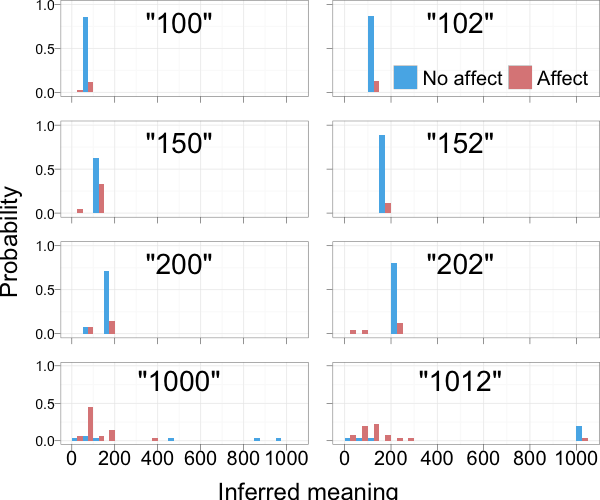
\includegraphics[width=0.65\textwidth]{humans_textbook_all.png}
	\caption{Human: Textbook costs}
\end{figure}

\begin{figure}[t]
	\centering
	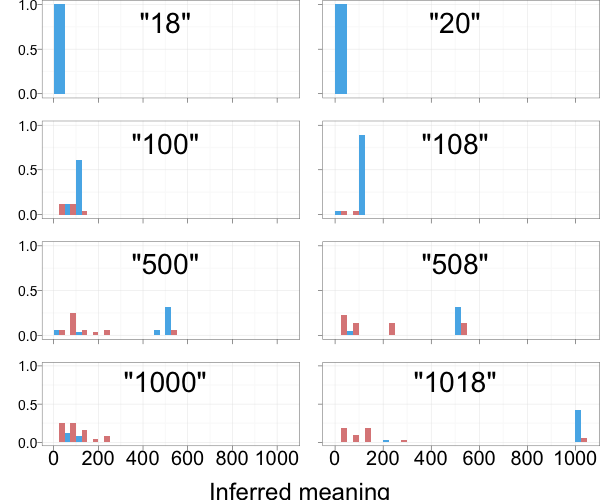
\includegraphics[width=0.65\textwidth]{humans_reading_all.png}
	\caption{Human: Length of reading assignments}
\end{figure}

\begin{figure}[t]
	\centering
	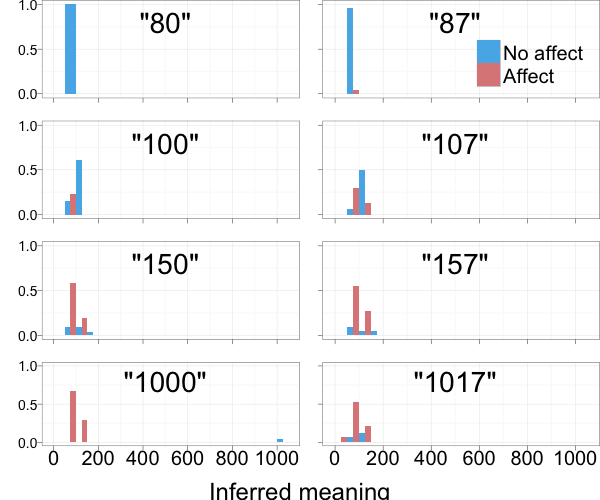
\includegraphics[width=0.65\textwidth]{humans_weather_all.png}
	\caption{Human: Weather temperature}
\end{figure}

\begin{figure}[t]
	\centering
	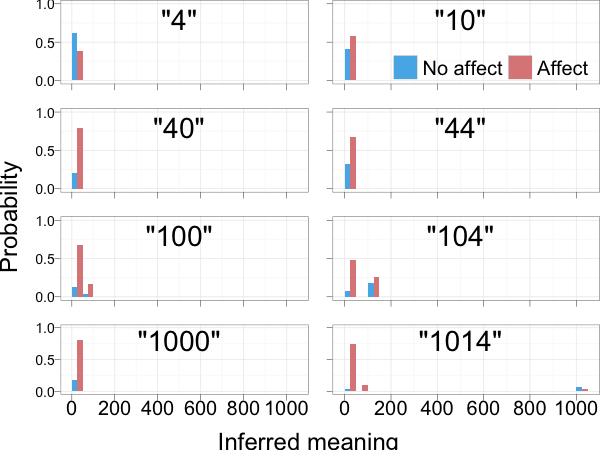
\includegraphics[width=0.65\textwidth]{humans_bus_all.png}
	\caption{Human: Bus wait time}
\end{figure}

\begin{figure}[t]
	\centering
	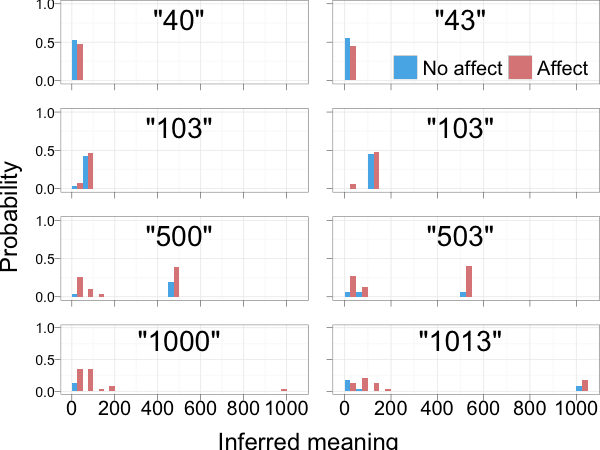
\includegraphics[width=0.65\textwidth]{humans_ticket_all.png}
	\caption{Human: Parking ticket costs}
\end{figure}

\end{document}
